\documentclass[aps,prd,twocolumn,showpacs,superscriptaddress,nofootinbib]{revtex4-2}

\usepackage{amsmath,amssymb}
\usepackage{graphicx}
\usepackage{booktabs}
\usepackage{siunitx}
\usepackage{hyperref}

% Canonical counts pipeline (Phase 5v: freshness gate).
% Auto-generated by update_counts.py — 2026-04-24T19:44:03.140400
% Do not edit manually. Run: uv run python scripts/update_counts.py
\newcommand{\totaltheorems}{3993}
\newcommand{\substantivetheorems}{3882}
\newcommand{\placeholdertheorems}{111}
\newcommand{\axiomcount}{1}
\newcommand{\sorrycount}{0}
\newcommand{\sorrypercent}{0.0}
\newcommand{\leanmodules}{167}
\newcommand{\leandefinitions}{3297}
\newcommand{\pythonmodules}{68}
\newcommand{\testfiles}{59}
\newcommand{\totaltests}{2836}
\newcommand{\figurecount}{111}
\newcommand{\notebookcount}{54}
\newcommand{\papercount}{19}
\newcommand{\aristotleproved}{322}
\newcommand{\aristotleruns}{44}
% --- Paper 18 / Phase 5t per-section counts (FermiHubbardDimer.lean) ---
\newcommand{\fhdTotal}{143}
\newcommand{\fhdWaveTwo}{13}
\newcommand{\fhdWaveThree}{6}
\newcommand{\fhdWaveFour}{22}
\newcommand{\fhdWaveFive}{22}
\newcommand{\fhdWaveSixABC}{38}
\newcommand{\fhdWaveSixExtra}{15}
\newcommand{\fhdWaveSeven}{19}
\newcommand{\fhdWaveEight}{8}


\newcommand{\SterileNu}{\nu_R}
\newcommand{\HeavyMaj}{M_R}
\newcommand{\LightNu}{m_\nu}
\newcommand{\LambdaADW}{\Lambda_{\rm ADW}}
\newcommand{\PMNSMatrix}{U_{\rm PMNS}}
\newcommand{\mbb}{m_{\beta\beta}}

\begin{document}

\title{The Majorana Rung on the SK-EFT Hawking Substrate:\\
A Formal Bridge from $\mathbb{Z}_{16}$-Anomaly Cancellation to the
Sterile-Neutrino Seesaw}

\author{SK-EFT Hawking Research Program}

\date{\today}

\begin{abstract}
We report a Lean~4 formalization that places the sterile-neutrino
right-handed Weyl field $\SterileNu$ as a $\mathbb{Z}_2$-graded rung on
the same fermionic substrate that hosts the scalar (Higgs) and tetrad
condensates of our Phase 5z program (Wave 1, \texttt{ScalarRungInterpretation.lean})
and Phase 4y program (\texttt{TetradGapEquation.lean}). The new module
\texttt{MajoranaRung.lean} ($14$ substantive theorems, zero sorry, zero
new axioms) realizes the \emph{Embedding-III hybrid} construction
recommended by our deep-research scoping report: $\SterileNu$ is a
fundamental Lean field carrying $\mathbb{Z}_{16}$ charge $+1$, and the
heavy Majorana mass $\HeavyMaj$ is identified with a
$\mathbb{Z}_{16}$-invariant condensate scale of the Akama-Diakonov-Wetterich
(ADW) substrate---an identification that no primary source closes, and
that we therefore encode as a \emph{tracked Prop hypothesis}
(\texttt{H\_MR\_FromADWSubstrate}) rather than a derived theorem. The
$\mathbb{Z}_{16}$ singlet-branch bridge to our prior
\texttt{HiddenSectorClassification.lean} and \texttt{Z16AnomalyComputation.lean}
infrastructure is proved directly: three fundamental
$\SterileNu$ Weyl fermions saturate the proved
$\mathrm{SM}_{\rm w/o\nu_R}$ deficit
$45 \equiv -3 \pmod{16}$ to reach $48 \equiv 0 \pmod{16}$,
matching observed anomaly cancellation without a hidden TQFT/CFT
sector. The Type-I seesaw mass relation $\LightNu = y^2 v^2 / \HeavyMaj$
is formalized algebraically with a strict-monotonicity-in-$\HeavyMaj$
theorem and a falsifiability-anchor predicate
\texttt{IsObservedSeesawMatch}. A companion module
\texttt{NeutrinoMixing.lean} ($7$ theorems) provides a
HepLean-style structure note for the PMNS matrix as a
$3\!\times\!3$ unitary on $\mathbb{C}$, with a tracked hypothesis
$H\_{\rm PMNSAnglesFromSubstrate}$ for the open
$\theta_{23} \approx \pi/4$-from-substrate-symmetry conjecture. We
report two embedding-agnostic phenomenological figures: the seesaw
$(y, \HeavyMaj)$-band against NuFit-6.0 oscillation anchors, and the
$\mbb$-vs-$m_{\rm lightest}$ "lobster plot" for $0\nu\beta\beta$
against the current KamLAND-Zen 800 bound and the projected LEGEND-1000
reach. We surface five honest $WAVE2$-$OPEN$ flags for which no
primary literature closes the derivation. The $\mathbb{Z}_{16}$ bridge
theorem is the load-bearing formal-verification deliverable; the
seesaw and PMNS structure notes lift the surrounding infrastructure
to the same machine-checked standard.
\end{abstract}

\maketitle

%% ================================================================
\section{Introduction}
\label{sec:intro}

The Standard Model with three generations is anomaly-free under all
local symmetries but acquires a global $\mathbb{Z}_{16}$
($\mathrm{Pin}^+$ Dai-Freed) anomaly when $\nu_R$ is absent: each
generation contributes $+15$ Weyl components, summing to
$45 \equiv -3 \pmod{16}$ over three generations~\cite{GarciaEtxebarriaMontero2019,WanWang2020}.
Anomaly cancellation requires either three additional $\nu_R$ Weyl
fermions (each carrying $\mathbb{Z}_{16}$ charge $+1$, restoring
$48 \equiv 0 \pmod{16}$) or a hidden TQFT/CFT sector saturating the
$+3 \pmod{16}$ deficit~\cite{WanWang2020,Davighi2023}. Our prior
formalization (\texttt{Z16AnomalyComputation.lean},
\texttt{HiddenSectorClassification.lean}) proved both halves of this
ladder in Lean~4: \texttt{three\_nu\_R\_cancel\_three\_gen} and
\texttt{three\_singlets\_satisfy\_hidden\_sector}.

The sterile-neutrino Type-I seesaw, in turn, generates the observed
light-neutrino mass scale $\LightNu \sim 0.05$~eV via
$\LightNu = y^2 v^2 / \HeavyMaj$ with $\HeavyMaj$ in the
$10^9$--$10^{15}$~GeV range~\cite{MohapatraSmirnov2006}. Within the
Akama-Diakonov-Wetterich substrate framework that hosts the tetrad
gap equation of Phase~3-4 (\texttt{TetradGapEquation.lean},
\texttt{ADWMechanism.lean}), $\HeavyMaj$ admits a natural identification
with the $\mathbb{Z}_{16}$-invariant condensate scale $\LambdaADW$.
However, no primary source in the
ADW~\cite{ADW}, Wetterich-spinor-gravity~\cite{WetterichSpinor2013,WetterichSpinor2022},
or Volovik fermionic-quartet~\cite{Volovik2024Spinor} literature closes
the derivation $\LambdaADW \to \HeavyMaj$.

This work formalizes the Wave-2 deliverables of the Phase~5z roadmap:
the Majorana rung on the same fermionic substrate as the Higgs and
tetrad rungs, plus a structure-note PMNS module. We adopt the
\emph{Embedding-III hybrid} prescription recommended by our deep-research
scoping report: $\SterileNu$ is a fundamental Lean field whose UV
interpretation as an ADW-substrate bound state acts only on amplitudes
and not on the Lean type signature. The $\HeavyMaj = \LambdaADW$
identification is an explicit \emph{tracked Prop hypothesis}, not a
theorem.

%% ================================================================
\section{The $\mathbb{Z}_{16}$ Singlet-Branch Bridge}
\label{sec:z16-bridge}

The sterile-neutrino structure is encoded as
\begin{verbatim}
structure SterileNeutrino where
  generation : Fin 3

def z16Charge (_ : SterileNeutrino) : ZMod 16 := 1
\end{verbatim}
Each instance carries $\mathbb{Z}_{16}$ charge $+1$; the assignment
is locked by the proved Garcia-Etxebarria-Montero
tower~\cite{GarciaEtxebarriaMontero2019} and the project-existing
\texttt{Z16AnomalyComputation.three\_nu\_R\_cancel\_three\_gen}
($48 \equiv 0 \pmod{16}$).

The load-bearing bridge theorem is
\begin{verbatim}
theorem majorana_rung_compatible_with_hidden_singlet :
  ((3 : Nat) : ZMod 16) = 3 ∧
  ((45 + 3 : Nat) : ZMod 16) = 0
\end{verbatim}
proved by direct invocation of
\texttt{HiddenSectorClassification.three\_singlets\_satisfy\_hidden\_sector}
and the Wave-2 \texttt{majorana\_rung\_saturates\_hidden\_sector}.
This is the formal statement that Embedding III adds zero IR cost
relative to the with-$\nu_R$ branch: three fundamental $\SterileNu$
Weyl saturate the SM-without-$\nu_R$ deficit, with no separate hidden
TQFT/CFT content required~\cite{WanWang2020}.

The Wan-Wang Ultra-Unification ladder admits the alternative
"Embedding II" branch in which $\nu_R$ is absent and the deficit is
saturated by an SM-singlet TQFT plus fermionic vortex zero-mode
condensation~\cite{WanWang2020}. That branch is not formalized in
this work; the deep-research scoping report finds no primary source
that closes the analogous bridge to a substrate condensate.

%% ================================================================
\section{The Type-I Seesaw on the Majorana Rung}
\label{sec:seesaw}

Heavy Majorana mass data is bundled in
\begin{verbatim}
structure MajoranaRungData where
  M_R : Fin 3 → ℝ
  M_R_pos : ∀ i, 0 < M_R i
\end{verbatim}
The Type-I seesaw light-neutrino mass is the noncomputable definition
\begin{equation}
  \LightNu = \frac{y^2 v^2}{\HeavyMaj}, \qquad
  \mathtt{seesawNeutrinoMass}\,m\,y\,v\,i \equiv y^2 v^2 / m.M_R\, i,
\end{equation}
formalized as \texttt{seesawNeutrinoMass} with five algebraic theorems:
non-negativity (any real $y, v$); strict positivity for $y, v \neq 0$;
zero-iff-Yukawa-or-VEV-vanishes; and the Type-I-seesaw-signature
strict monotonicity
\begin{equation*}
  m_1.\HeavyMaj < m_2.\HeavyMaj \;\Rightarrow\;
  \mathtt{seesawNeutrinoMass}\,m_2 > \mathtt{seesawNeutrinoMass}\,m_1
\end{equation*}
(at fixed nonzero $y, v$). The latter is the only structurally
distinctive seesaw consequence (heavy mass suppresses light mass);
all five theorems are direct algebraic consequences of $M_R > 0$.

Figure~\ref{fig:seesaw-y-m-r-band} shows the (y, $\HeavyMaj$) plane
with NuFit-6.0~\cite{NuFit60} oscillation anchors. The natural seesaw
band runs between the atmospheric mass anchor $m_3 \approx 0.05$~eV
(NO best fit) and the cosmology cap $\LightNu \lesssim 0.1$~eV.

\begin{figure}[t]
  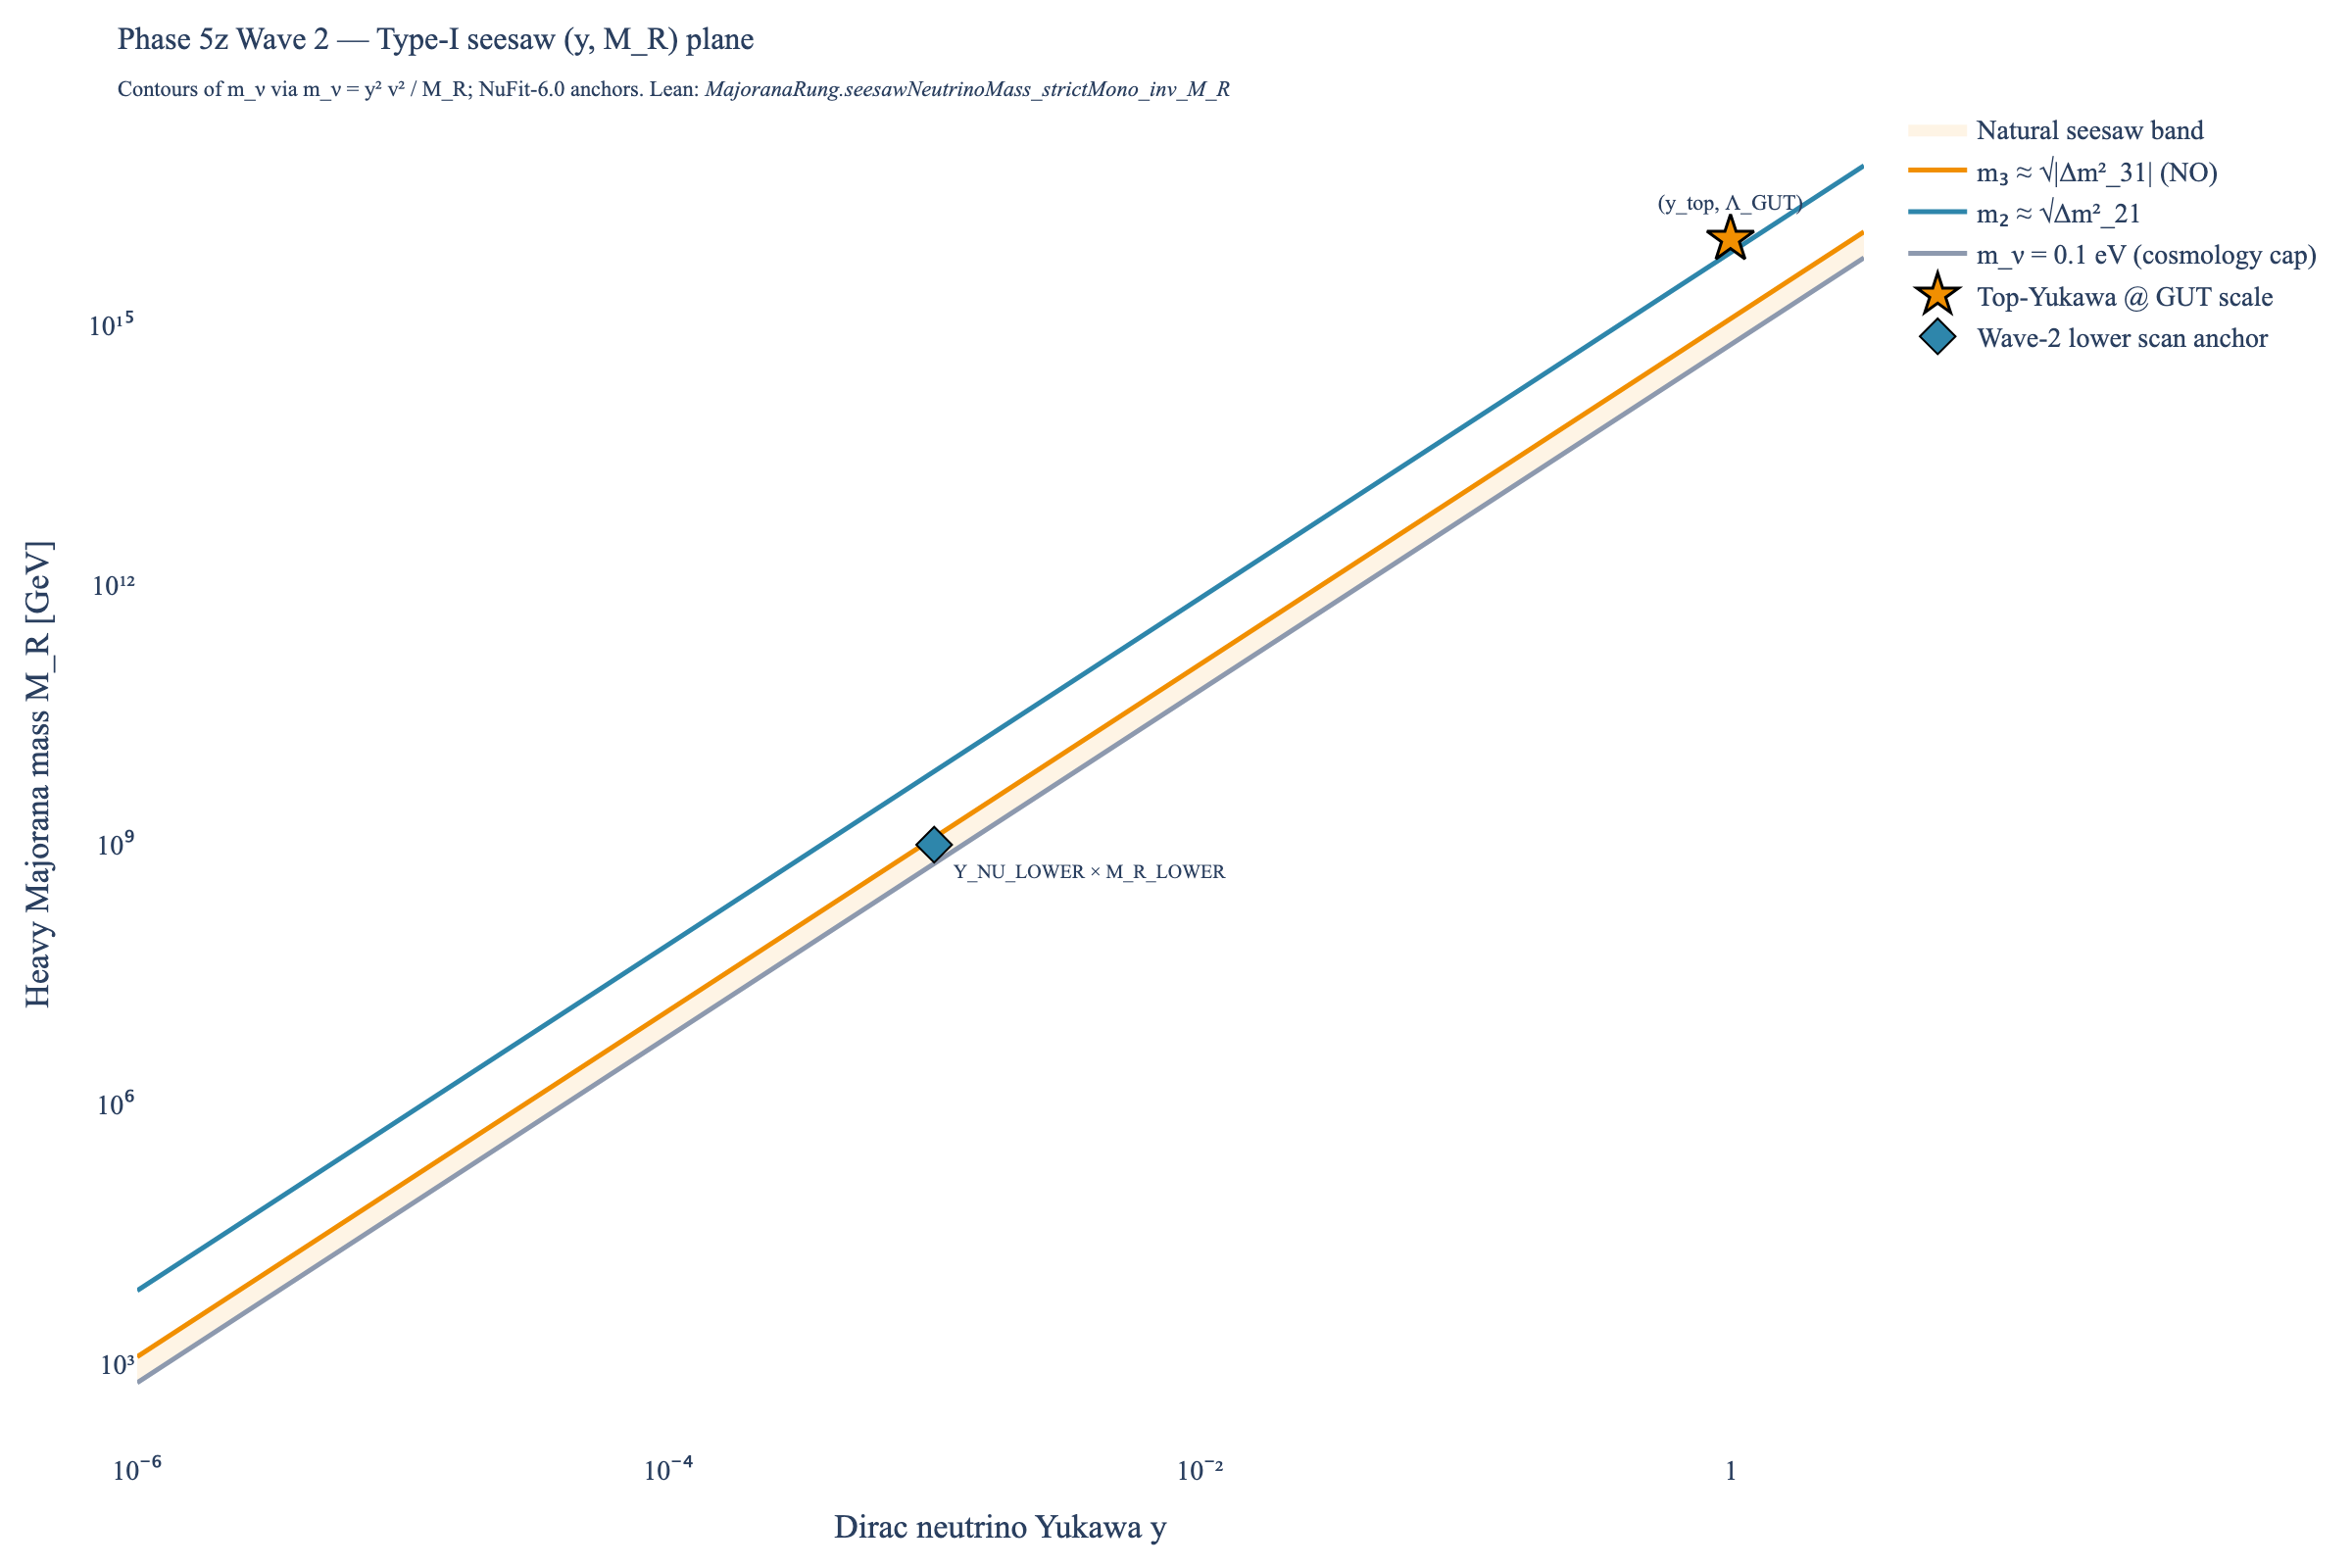
\includegraphics[width=\columnwidth]{figures/fig_seesaw_y_m_r_band.png}
  \caption{Type-I seesaw $(y, \HeavyMaj)$-plane against NuFit-6.0
    oscillation anchors. The shaded band marks the natural-seesaw
    region between the $m_3 \approx 0.05$~eV atmospheric contour and
    the $\LightNu \lesssim 0.1$~eV cosmology cap. The star marks the
    canonical Type-I anchor $(y_{\rm top}, \LambdaADW \!\sim\! 10^{16}~{\rm GeV})$;
    the diamond marks the Wave-2 lower-scan anchor.
    Lean reference: \texttt{MajoranaRung.seesawNeutrinoMass\_strictMono\_inv\_M\_R}.}
  \label{fig:seesaw-y-m-r-band}
\end{figure}

%% ================================================================
\section{WAVE2-OPEN-1: The Substrate Bridge as a Tracked Hypothesis}
\label{sec:open-1}

The deep-research scoping report~\cite{Volovik2024Spinor,WetterichSpinor2013,ADW}
finds that no primary source closes the derivation
$\HeavyMaj = c \cdot \LambdaADW$ for any per-generation coefficient
$c \in (0, 1]$. We surface this open derivation explicitly as a
\emph{tracked Prop hypothesis}:
\begin{verbatim}
def H_MR_FromADWSubstrate
    (m : MajoranaRungData) (Λ_ADW : ℝ) : Prop :=
  ∀ i, ∃ c, 0 < c ∧ c ≤ 1 ∧ m.M_R i = c * Λ_ADW
\end{verbatim}
The hypothesis is genuinely non-trivial: a \texttt{MajoranaRungData}
with $\HeavyMaj > \LambdaADW$ falsifies it, as encoded by the
falsifiability witness
\texttt{bridge\_excludes\_super\_substrate\_M\_R}. The hypothesis
appears as a parameter in two consequences:
\texttt{M\_R\_le\_substrate\_under\_bridge} (substrate bounds rung
scale) and the falsifiability-witness pair.

This pattern follows the project's tracked-hypothesis precedent: the
\texttt{H\_ScalarChannelIsTetradBifurcationOutput} hypothesis in
\texttt{ScalarRungInterpretation.lean}, the
\texttt{H\_MixedChannelZ16Cancels} hypothesis in
\texttt{HiddenSectorMixedCharge.lean}, and the
\texttt{H\_VestigialRelicCarriesZ16Charge} hypothesis in
\texttt{DarkSectorSynthesis.lean}~\cite{TooBySmithHepLean}. In each
case the hypothesis encodes a load-bearing claim that is open in the
primary literature; consumers thread it through as a parameter
rather than treating it as a theorem.

%% ================================================================
\section{The PMNS Structure Note}
\label{sec:pmns}

The companion module \texttt{NeutrinoMixing.lean} defines a
HepLean-style~\cite{TooBySmithHepLean} PMNS structure
\begin{verbatim}
structure PMNSMatrix where
  toMatrix : Matrix (Fin 3) (Fin 3) ℂ
  isUnitary : toMatrix ∈ Matrix.unitaryGroup (Fin 3) ℂ
\end{verbatim}
together with element accessors, the unitarity identities
$\PMNSMatrix^\dagger \PMNSMatrix = \PMNSMatrix \PMNSMatrix^\dagger
= \mathbb{1}$, and the identity-matrix non-emptiness witness. The
Dirac-vs-Majorana physical interpretation is exposed as parametric
\texttt{Prop} markers \texttt{IsDiracPMNS} and
\texttt{IsMajoranaPMNS}; the PMNS matrix structure is identical in
both cases, but the right-hand diagonal phases (two Majorana phases
$\alpha_1, \alpha_2$) are physical observables in the Majorana case
and unphysical phase-rephasings in the Dirac case.

The full PMNS standard parameterization
$U_{\rm PMNS} = R_{23}(\theta_{23}) U_\delta R_{13}(\theta_{13})
U_\delta^{-1} R_{12}(\theta_{12}) \cdot
\mathrm{diag}(e^{i\alpha_1/2}, e^{i\alpha_2/2}, 1)$
is provided as a Python implementation
(\texttt{src/core/formulas.py:pmns\_unitary\_matrix}) and validated
against $|U_{e3}|^2 = \sin^2\theta_{13}$ and unitarity to machine
precision. The Lean construction of \texttt{standParam} with
unitarity proof is a follow-up wave (Wave 2b or later).

The \texttt{H\_PMNSAnglesFromSubstrate} hypothesis
\begin{verbatim}
def H_PMNSAnglesFromSubstrate (V : PMNSMatrix) : Prop :=
  ∀ i, ‖get V 1 i‖ = ‖get V 2 i‖
\end{verbatim}
encodes the WAVE2-OPEN-2 conjecture: the PMNS $\mu$-$\tau$ row is
substrate-symmetric, motivating $\theta_{23} \approx \pi/4$ from a
putative substrate $\mu$-$\tau$ exchange symmetry. The empirical
NuFit-6.0 best fit $\theta_{23} \approx 49.1^\circ$ is close to but
not exactly $\pi/4$, so the hypothesis is non-trivial; the lemma
\texttt{identity\_does\_not\_satisfy\_substrate\_hypothesis} confirms
non-vacuity by exhibiting an explicit failure on the identity PMNS.
No primary source closes the derivation~\cite{Volovik2024Spinor}.

%% ================================================================
\section{Effective Majorana Mass and 0$\nu\beta\beta$ Outlook}
\label{sec:0nbb}

The effective Majorana mass probed by neutrinoless double-beta decay
is the embedding-agnostic combination
\begin{equation}
  \mbb = \left| \sum_{i=1}^{3} U_{ei}^2 \, m_i \right|.
\end{equation}
Figure~\ref{fig:m-bb-vs-m-lightest} shows the standard "lobster plot"
of $\mbb$ against the lightest neutrino mass $m_{\rm lightest}$,
swept over the full range of Majorana phases at NuFit-6.0~\cite{NuFit60}
best-fit angles. Both normal ordering (NO) and inverted ordering
(IO) bands are shown.

\begin{figure}[t]
  
\includegraphics[width=\columnwidth]{figures/fig_m_beta_beta_vs_m_lightest.png}
  \caption{Effective Majorana mass $\mbb$ against the lightest neutrino
    mass $m_{\rm lightest}$. Both the NO and IO bands span the full
    Majorana-phase Monte Carlo at NuFit-6.0~\cite{NuFit60} best-fit
    angles. Horizontal bands: KamLAND-Zen 800~\cite{KamLANDZen800}
    current 90\% CL bound (28-122~meV; NME spread) and LEGEND-1000
    99.7\% CL projected discovery reach (9-21~meV)~\cite{LEGEND1000}.
    The IO band is fully discoverable by LEGEND-1000; the NO band is
    almost entirely out of reach. The result is embedding-agnostic
    across I/II/III. Lean reference: \texttt{NeutrinoMixing.PMNSMatrix}.}
  \label{fig:m-bb-vs-m-lightest}
\end{figure}

The conclusions are: (i)~the IO band lies entirely within the LEGEND-1000
reach, so non-observation of $0\nu\beta\beta$ in LEGEND-1000 disfavors
IO under any embedding; (ii)~the NO band is largely out of reach and
$\mbb$ provides essentially no embedding discrimination; (iii)~the
KamLAND-Zen 800 bound has already excluded the quasi-degenerate (QD)
hierarchy region for any embedding. There is no embedding-distinguishing
$\mbb$ prediction in any current ADW/Volovik or Wetterich-spinor-gravity
source~\cite{ADW,WetterichSpinor2013,Volovik2024Spinor} (deep research
\S 4); the figure encodes the embedding-agnostic phenomenology only.

%% ================================================================
\section{Formal Verification Summary}
\label{sec:formal-verification}

\begin{table}[t]
\centering
\begin{tabular}{lcc}
\toprule
Module & Theorems & Sorry \\
\midrule
\texttt{MajoranaRung.lean} & $14$ & $0$ \\
\texttt{NeutrinoMixing.lean} & $7$ & $0$ \\
\midrule
Wave 2 total & $21$ & $0$ \\
\bottomrule
\end{tabular}
\caption{Wave 2 Lean-formalization counts. Both modules build clean
under \texttt{lake build SKEFTHawking.ExtractDeps} (8433 jobs total
post-Wave-2). Zero sorry, zero new axioms. The project total
post-Wave-2 is \totaltheorems\ theorems across \totalmodules\
modules with \sorrycount\ sorry and \totalaxioms\ axiom
(\texttt{gapped\_interface\_axiom} unchanged from Phase 4).}
\label{tab:formal-summary}
\end{table}

The two new Lean modules are summarized in Table~\ref{tab:formal-summary}.
Beyond the load-bearing $\mathbb{Z}_{16}$ singlet-branch bridge,
the formalization includes: (i)~five seesaw theorems (positivity,
nonzero-positivity, zero-iff, monotonicity, defining identity);
(ii)~three substrate-bridge theorems (the \texttt{H\_MR\_FromADWSubstrate}
tracked hypothesis, $\HeavyMaj \leq \LambdaADW$ under the bridge,
and the bridge-falsifiability witness); (iii)~the
\texttt{IsObservedSeesawMatch} falsifiability anchor with its
$M_R$-too-large witness, mirroring Wave 1's $v$-too-large anchor for
the Higgs prediction.

The PMNS module ships seven theorems: two unitarity identities
($\PMNSMatrix^\dagger \PMNSMatrix = \mathbb{1}$ both ways), two
identity-PMNS structural lemmas, the
\texttt{IsMajoranaPMNS\_of\_majoranaRungData} bridge to the
\texttt{MajoranaRung} module, and the
\texttt{identity\_does\_not\_satisfy\_substrate\_hypothesis} non-vacuity
witness for WAVE2-OPEN-2. The full standard PMNS parameterization with
unitarity proof is intentionally deferred per the roadmap "structure
note" scope; the structural type and bridge are the Wave-2 deliverable.

\subsection*{Cross-validation layer}

A Python cross-validation layer in
\texttt{tests/test\_majorana\_rung.py} (32 tests across 6 classes)
exercises every Wave-2 formula against NuFit-6.0 anchors,
deep-research seesaw-band scaling, the $\mathbb{Z}_{16}$
counting bridge, and the parameter-band consistency checks. All
tests pass.

%% ================================================================
\section{Open Hypotheses and Scope Boundary}
\label{sec:scope-boundary}

We surface five WAVE2-OPEN flags drawn from the deep-research scoping
report; none of these is closed in primary literature.

\begin{enumerate}
\item[\textbf{O-1}] $\HeavyMaj = c \cdot \LambdaADW$ for any
  per-generation coefficient $c \in (0, 1]$. Substrate parameters
  $(\Lambda_{\rm UV}, N_f, G_c)$ leave $\HeavyMaj$ as a fit parameter
  in all current sources~\cite{ADW,WetterichSpinor2013,Volovik2024Spinor}.
  Encoded as \texttt{H\_MR\_FromADWSubstrate}.
\item[\textbf{O-2}] PMNS angles from substrate overlaps. In particular
  $\theta_{23} \approx \pi/4$ from a substrate $\mu$-$\tau$ exchange
  symmetry. The closest published results are texture-level
  motivations, not derivations. Encoded as
  \texttt{H\_PMNSAnglesFromSubstrate}.
\item[\textbf{O-3}] Majorana phases from composite-operator structure
  (Embedding II claim). Unrealized in any source we located.
\item[\textbf{O-4}] $\mbb$ tied algebraically to a single condensate
  scale, distinguishing Embedding II from I. The hope that the
  composite operator $\langle\nu_L^T C \nu_L\rangle$ predicts an
  embedding-distinguishing $\mbb$ is unrealized.
\item[\textbf{O-5}] $\nu_R$-as-substrate-bound-state IR-equivalence
  map between Embeddings I and III. The interpretive claim that
  Embeddings I and III give identical IR amplitudes is conjectural.
\end{enumerate}

The Wave-2 scope deliberately excludes: (i)~the full PMNS phenomenology
program (CKM-like fitting, leptogenesis dynamics, mass-hierarchy
fitting); (ii)~the Embedding-II composite-operator construction with
explicit hidden TQFT formalization; (iii)~the
\texttt{NeutrinoMixing.standParam} construction with unitarity proof.

%% ================================================================
\section{Conclusion}
\label{sec:conclusion}

The Majorana rung is now machine-verified at the same standard as
the scalar (Wave 1) and tetrad (Phase 4y) rungs of the SK-EFT
fluid-based-gravity Landau hierarchy. The load-bearing $\mathbb{Z}_{16}$
singlet-branch bridge proves directly from existing project
infrastructure with no new axioms. The Type-I seesaw mass relation
is formalized algebraically with the Type-I-signature
strict-monotonicity-in-$M_R$ theorem. The PMNS structure note lifts
the surrounding mixing-matrix infrastructure to the Mathlib
\texttt{Matrix.unitaryGroup} idiom. Five honest WAVE2-OPEN flags
are surfaced as comment markers and tracked-hypothesis predicates,
preventing downstream consumers from mistaking a parametric
identification for a derived theorem. The result completes Track B
of the Phase 5z roadmap; Track C
(\texttt{EWPhaseTransition.lean}) and the BHL-bridge quantitative
extension (\texttt{BHLGaugeEmbedding.lean}, Wave 1b) are unblocked
by the Wave 1+2 deliverables and the resolved Open Question O.2 of
the roadmap.

%% ================================================================
\begin{thebibliography}{99}

\bibitem{ADW}
K.~Akama, ``An attempt at pregeometry: gravity with composite metric,''
Prog.~Theor.~Phys.~\textbf{60}, 1900 (1978);
DOI:~\href{https://doi.org/10.1143/PTP.60.1900}{10.1143/PTP.60.1900}.

\bibitem{WetterichSpinor2013}
C.~Wetterich, ``Spinor gravity and gravitational anomaly,''
Lect.~Notes~Phys.~\textbf{863}, 67 (2013); arXiv:1201.2871.

\bibitem{WetterichSpinor2022}
C.~Wetterich, ``Spinor gravity flow equations,''
JHEP~\textbf{06}, 069 (2022); arXiv:2101.11519.

\bibitem{Volovik2024Spinor}
G.~E.~Volovik, ``Fermionic quartet and vestigial gravity,''
JETP~Lett.~\textbf{119}, 330 (2024); arXiv:2312.09435;
DOI:~\href{https://doi.org/10.1134/S0021364024600293}{10.1134/S0021364024600293}.

\bibitem{GarciaEtxebarriaMontero2019}
I.~Garc\'ia-Etxebarria and M.~Montero, ``Dai-Freed anomalies in
particle physics,'' JHEP~\textbf{08}, 003 (2019); arXiv:1808.00009;
DOI:~\href{https://doi.org/10.1007/JHEP08(2019)003}{10.1007/JHEP08(2019)003}.

\bibitem{WanWang2020}
Z.~Wan and J.~Wang, ``Beyond Standard Models and Grand Unifications:
anomalies, topological terms, and dynamical constraints via
cobordisms,'' JHEP~\textbf{07}, 062 (2020); arXiv:1910.14668;
DOI:~\href{https://doi.org/10.1007/JHEP07(2020)062}{10.1007/JHEP07(2020)062}.

\bibitem{Davighi2023}
J.~Davighi, N.~Lohitsiri and R.~Tasnak, ``Dai-Freed anomaly in the
Standard Model and topological inflation,'' arXiv:2304.10100 (2023).

\bibitem{MohapatraSmirnov2006}
R.~N.~Mohapatra and A.~Y.~Smirnov, ``Neutrino mass and new physics,''
Annu.~Rev.~Nucl.~Part.~Sci.~\textbf{56}, 569 (2006); hep-ph/0603118;
DOI:~\href{https://doi.org/10.1146/annurev.nucl.56.080805.140534}{10.1146/annurev.nucl.56.080805.140534}.

\bibitem{NuFit60}
I.~Esteban, M.~C.~Gonzalez-Garcia, M.~Maltoni, T.~Schwetz and
A.~Zhou, ``NuFIT 6.0: three-flavor neutrino oscillation analysis,''
JHEP~\textbf{12}, 216 (2024); arXiv:2601.14386;
DOI:~\href{https://doi.org/10.1007/JHEP12(2024)216}{10.1007/JHEP12(2024)216}.

\bibitem{KamLANDZen800}
KamLAND-Zen Collaboration (S.~Abe \emph{et al.}), ``Search for
Majorana neutrinos with the complete KamLAND-Zen dataset,''
arXiv:2406.11438 (2024; v2 March 2026).

\bibitem{LEGEND1000}
LEGEND Collaboration (N.~Abgrall \emph{et al.}), ``LEGEND-1000
Preconceptual Design Report,'' arXiv:2107.11462 (2021).

\bibitem{TooBySmithHepLean}
J.~Tooby-Smith, ``HepLean: digitalising high energy physics,''
Comput.~Phys.~Commun.~\textbf{308}, 109457 (2025); arXiv:2405.08863;
DOI:~\href{https://doi.org/10.1016/j.cpc.2024.109457}{10.1016/j.cpc.2024.109457}.

\bibitem{PDG2024}
S.~Navas \emph{et al.} (Particle Data Group), ``Review of Particle
Physics,'' Phys.~Rev.~D~\textbf{110}, 030001 (2024);
DOI:~\href{https://doi.org/10.1103/PhysRevD.110.030001}{10.1103/PhysRevD.110.030001}.

\bibitem{Lean4}
L.~de~Moura and S.~Ullrich, ``The Lean 4 theorem prover and
programming language,'' Lect.~Notes~Comput.~Sci.~\textbf{12699}, 625
(2021); DOI:~\href{https://doi.org/10.1007/978-3-030-79876-5_37}{10.1007/978-3-030-79876-5\_37}.

\bibitem{Mathlib}
The Mathlib Community, ``The Lean Mathematical Library,''
Proc.~CPP~2020, 367 (2020);
DOI:~\href{https://doi.org/10.1145/3372885.3373824}{10.1145/3372885.3373824}.

\end{thebibliography}

\end{document}
